\documentclass{article}

\usepackage[T1]{fontenc}
\usepackage[polish]{babel}
\usepackage[utf8]{inputenc}
\usepackage{float}
\usepackage{graphicx}
\usepackage{amsmath}
\usepackage{siunitx}
\oddsidemargin 0pt
\evensidemargin 0pt
\marginparwidth 40pt
\marginparsep 10pt
\topmargin -20pt
\headsep 10pt
\textheight 8.7in
\textwidth 6.65in
\linespread{1.2}

\title{Sprawozdanie z Laboratorium 4. \\ \large Pomiar stężenia radonu}
\author{Piotr Lewandowski \and Dymitr Lubczyk \and Krzysztof Tabeau}
\date{\today}

\begin{document}
\maketitle
\clearpage
\section{Część teoretyczna}
Jest to część poświęcona omówieniu zagadnień związanych z przeprowadzonym doświadczeniem oraz przedstawieniu układu doświadczalnego.
\subsection{Wstęp}
Celem dzisiejszego doświadczenia było wyznaczenie stężenia Radonu. Radon jest radioaktywnym gazem szlachetnym powstałym z rozpadu Radu.
Jego najstabilniejszy izotop ma czas połowicznego rozpadu wynoszący nie co mniej niż 4 dni. Ale co jest najistotniejsze to fakt, że Radon emituje promieniowanie $\alpha$, które będzie kluczowe dla zmierzenia  stężenia Radonu w powietrzu. Ze względu na istotność tego promieniowania w naszym doświadczeniu pozwolimy sobie je pokrótce przedstawić. Jest to promieniowanie pojawiające się w wyniku rozpadu jądra atomowego, jądro to emituje cząstkę $\alpha$ będącą identyczną z atomem helu, jest to promieniowanie bardzo silnie absorbowane przez materię, gdyż już kartka papieru jest wystarczająca, żeby osłonić nas przed tym promieniowaniem.
\subsection{Opis układów doświadczalnych}
W doświadczeniu chcemy wyznaczyć stężenie Radonu którym zostały naświetlone detektory śladowe - płytki PADC. W tym celu wykorzystując program ImageJ analizujemy 10 zdjęć tych płytek wykonanych pod mikroskopem.


\section{Część doświadczalna}
Jest to część poświęcona przedstawieniu zebranych wyników, przeprowadzeniu analizy ich niepewności pomiarowych jak i przestawieniu finalnego rezultatu
\subsection{Wykonane pomiary}
Poniżej widzimy tabelkę z pomiarami średnicy, pomiary zostały wykonane łącznie 30 razy:

\begin{table}[h!]
\centering
\begin{tabular}{|l|l|l|}
\hline
1.382	& 1.385	& 1.387 \\
1.39	& 1.389	& 1.391 \\
1.384	& 1.377	& 1.381 \\
1.384	& 1.378	& 1.378 \\
1.384	& 1.379	& 1.383 \\
1.38	& 1.383	& 1.377 \\
1.384	& 1.388	& 1.386 \\
1.386	& 1.384	& 1.382 \\
1.386	& 1.386	& 1.385 \\
1.385	& 1.385	& 1.385 \\
\hline
\end{tabular}
\end{table}

\clearpage


Poniżej widzimy tabelkę z pomiarami liczby otworów na badanej przez nas płytce PADC, pomiar został wykonany 21 razy:

\begin{table}[h!]
\centering
\begin{tabular}{|l|l|l|}
\hline
105	& 98	& 118 \\
109	& 139	& 155 \\
96	& 110	& 140 \\
97	& 96	& 84 \\
56	& 119	& 81 \\
74	& 139	& 145 \\
122	& 176	& 161 \\
\hline
\end{tabular}
\end{table}

\begin{figure}[h!]
\centerline{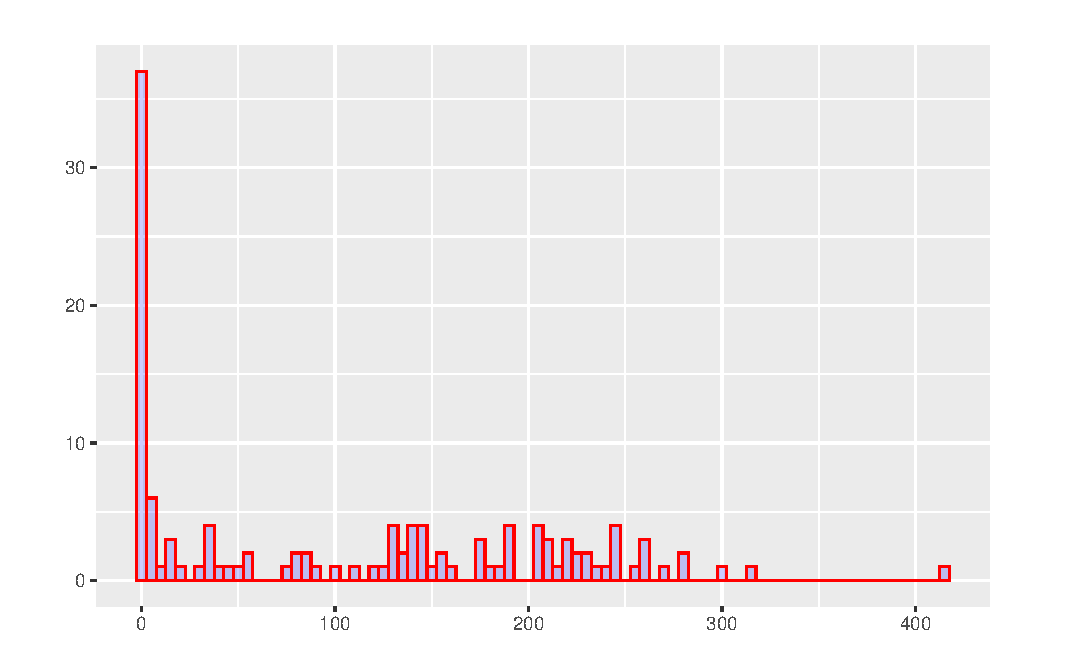
\includegraphics[scale=1]{Fizyka4}}
\caption{histogram wielkości pól dziurek $\SI{}{\micro\metre}^2$ w płytce dla jednego zdjęcia}
\end{figure}

\clearpage

\subsection{Opracowanie wyników}
W celu wyznaczenia niepewności pomiarowej pola powierzchni płytki posłużyliśmy się metodą propagacji błędu otrzymując poniższe równania:
\begin{gather*}
p = \pi (d/2)^2 \\
u(p)=\sqrt{\frac{\partial P}{\partial d}^2 u(d)^2 }\\
u(p)=|\frac{\pi d}{2}u(d)|
\end{gather*}
gdzie u(d) to niepewność pomiarowa średnicy. Zgodnie z instrukcją zakładamy, że jest on równa odchyleniu standardowemu średniej, więc wartość średnicy wynosi: $1.3835(25) mm$. Wykorzystując powyższe wzory możemy wywnioskować, że pole powierzchni to $1.5049(79) mm^2$. \\
Średnia liczba otworów na płytce to, według naszych pomiarów, 103.17(14.75), co daje nam 68.6(9.80) dziurek na $mm^2$ \\\
Niepewność liczby otworów wyznaczyliśmy zgodnie z instrukcją ćwiczenia i otrzymaliśmy wartość 14,3\% \\
Za pomocą poniższego wzoru na stężenie radonu na 90 dni 
$$
4.11(36)[\frac{Bq/m^3}{n/mm^2}] * \rho + 46.9(23.4)[Bq/m^3]
$$
możemy łatwo policzyć, że stężenie radonu w powietrzu wynosi 328.846(91.9) [Bq/m\^3]
\subsection{Podsumowanie}
Wynik eksperymentu wyszedł stosunkowo mały co do typowego stężenia radonu. Można nawet postawić hipotezę, że zdjęcia płytki były wykonywane latem lub w budynku na względnie wysokiej kondygnacji, ponieważ statystycznie wtedy wyniki są mniejsze. Niestety na zdjęciach, które otrzymaliśmy do przeprowadzenia tego badania były wyraźnie widoczne uszkodzenia mechaniczne mikroskopu. Na niekorzyść działa również jakość kamery w telefonie, którym te zdjęcia były robione. Z dziesięciu zdjęć w paczce danych niestety musieliśmy odrzucić trzy, ponieważ mogłyby mocno zwiększyć niepewność otrzymanych wyników.
\end{document}
